\documentclass[conference]{IEEEtran}

\usepackage[utf8]{inputenc}
\usepackage[T1]{fontenc}
\usepackage{amsmath,amssymb,amsfonts}
\usepackage{graphicx}
\usepackage{booktabs}
\usepackage{array}
\usepackage{cite}
\usepackage{url}
\usepackage[hidelinks]{hyperref}

\begin{document}

\title{Training-Free Sentence-Level Context Pruning for Retrieval-Augmented Generation using Dual Sparse-Dense Scoring}

\author{
\IEEEauthorblockN{Anonymous Author(s)}
\IEEEauthorblockA{Department of Computer Science and Engineering\\
Institution Name\\
City, Country\\
email@institution.edu}
}

\maketitle

\begin{abstract}
Retrieval-Augmented Generation (RAG) grounds large language models (LLMs) in external evidence, yet imperfect first-stage retrievers frequently inject topically related distractor passages alongside the ground-truth context. On resource-constrained readers, these extraneous tokens inflate prefill latency and degrade span extraction via distractor interference and the ``Lost in the Middle'' phenomenon. Existing prompt-compression techniques either rely on auxiliary causal language models to compute token-level perplexity---introducing substantial compute overhead and fragmenting syntax---or require task-specific supervised fine-tuning. We propose \textbf{Training-Free Sentence-Level Context Pruning (TF-SCP)}, a lightweight, model-agnostic post-retrieval filter operating between the retriever and the reader. TF-SCP segments retrieved passages into sentences, scores each sentence against the query using min-max normalized sparse lexical matching (BM25Okapi) and dense semantic similarity (\texttt{all-MiniLM-L6-v2}), combines them through convex fusion $F(s_j) = \alpha \cdot \hat{s}_{\mathrm{lex}}(s_j) + (1 - \alpha) \cdot \hat{s}_{\mathrm{sem}}(s_j)$, and discards sentences falling below a distribution-aware dynamic threshold $\tau = \mu_F + \beta \cdot \sigma_F$. Evaluated on $n=1,000$ answerable SQuAD v2 queries augmented with mined BM25 hard-negative distractors using a local \texttt{Qwen2.5-0.5B-Instruct} reader, TF-SCP ($\alpha=0.5, \beta=0.0$) eliminates 55.79\% of context tokens while retaining 97.5\% of gold answers---rescuing 73.3\% of genuine lexical-only answer losses ($p = 2.6 \times 10^{-12}$)---and improves F1 by $+2.73$ points. Under precision-oriented thresholding ($\alpha=0.5, \beta=+0.5$), TF-SCP achieves 74.25\% token reduction, a 30.1\% end-to-end latency reduction on CPU, and Bonferroni-significant improvements of $+6.67$ F1 ($p = 0.0001$) and $+4.80$ Exact Match ($p = 0.0010$) over full-context RAG.
\end{abstract}

\begin{IEEEkeywords}
Retrieval-Augmented Generation, Context Pruning, Prompt Compression, Hybrid Retrieval, Sparse-Dense Fusion, Question Answering
\end{IEEEkeywords}

\section{Introduction}

Retrieval-Augmented Generation (RAG) mitigates parametric hallucination and knowledge staleness in large language models (LLMs) by conditioning generation on non-parametric evidence fetched from an external corpus~\cite{lewis2020rag,karpukhin2020dpr}. In practice, standard bi-encoder and sparse retrievers optimize recall over top-$k$ passages, meaning the retrieved context presented to the downstream generator routinely contains substantial off-target text alongside a small number of answer-bearing sentences~\cite{cuconasu2024noise}. Passing all retrieved documents verbatim into the reader prompt introduces two coupled bottlenecks. First, transformer prefill computation and hosted API billing scale directly with prompt length, inflating end-to-end latency on edge or CPU-bound deployments. Second, empirical studies demonstrate that LLMs struggle to exploit relevant spans buried within long or noisy contexts---exhibiting U-shaped positional sensitivity known as the ``Lost in the Middle'' effect~\cite{liu2024lost} and marked susceptibility to topically adjacent distractors~\cite{shi2023distracted}.

To alleviate context bloat, prior work has explored learned extractive compressors~\cite{xu2024recomp,wang2023filco} and perplexity-based token-level prompt pruning methods such as Selective Context~\cite{li2023selective}, LLMLingua~\cite{jiang2023llmlingua}, and LongLLMLingua~\cite{jiang2024longllmlingua}. While effective on large cloud models, these paradigms impose critical practical barriers: supervised compressors require in-domain training pairs and risk brittle out-of-distribution generalization, whereas perplexity-driven pruners require running an auxiliary autoregressive causal LM over the entire retrieved prompt, neutralizing latency gains on compact hardware and often excising syntactic glue or punctuation needed by small instruction-tuned readers. Conversely, purely heuristic sparse filtering using lexical overlap (e.g., sentence-level BM25) is fast and training-free, yet systematically drops valid evidence whenever queries paraphrase source terminology or bridge entities indirectly.

To resolve this accuracy--latency--complexity trade-off, we introduce \textbf{Training-Free Sentence-Level Context Pruning (TF-SCP)}. Operating as a drop-in middleware stage between any retriever and any reader LLM, TF-SCP preserves grammatical integrity by pruning at sentence granularity without training or auxiliary generative passes. By fusing query-local min-max normalized BM25 lexical scores with lightweight dense bi-encoder cosine similarities and filtering against an adaptive mean-plus-dispersion threshold ($\tau = \mu_F + \beta \cdot \sigma_F$), TF-SCP adapts automatically to each query's score landscape.

The primary contributions of this work are summarized as follows:
\begin{itemize}
    \item \textbf{Training-Free Dual Sparse-Dense Sentence Pruner (TF-SCP):} We formulate an end-to-end, zero-shot post-retrieval sentence filtering pipeline combining dependency-aware segmentation, query-local sparse-dense convex score fusion, and moment-based dynamic thresholding that preserves document boundaries and narrative order.
    \item \textbf{Rigorous Large-Scale Statistical Evaluation ($n=1,000$):} We evaluate TF-SCP across eight $(\alpha, \beta)$ operating points on 1,000 SQuAD v2 queries augmented with corpus-wide BM25 hard-negative paragraphs using a compact \texttt{Qwen2.5-0.5B-Instruct} reader on CPU, establishing statistical significance via 10,000-resample paired bootstrap tests, exact McNemar tests, and Bonferroni family-wise error correction ($\alpha_{\mathrm{FWER}} = 0.0071$).
    \item \textbf{Mechanistic Decomposition of Recall vs.\ Denoising:} We decompose net reader accuracy into an \emph{answer-recall preservation} term and a \emph{distractor denoising} term, proving empirically why aggressive hybrid thresholding ($\alpha=0.5, \beta=+0.5$) simultaneously delivers higher token compression (74.25\% vs.\ 63.71\%), higher answer retention (94.5\% vs.\ 93.2\%), and significantly higher QA accuracy ($+4.07$ F1, $p=0.0001$) than lexical-only pruning.
\end{itemize}

\section{Related Work}

\subsection{Context Length Overhead and Distractor Sensitivity in RAG}
Early open-domain RAG architectures such as RAG-Sequence/Token~\cite{lewis2020rag} and Fusion-in-Decoder (FiD)~\cite{izacard2021fid} established that conditioning generation on retrieved passages from dense encoders~\cite{karpukhin2020dpr} substantially boosts factual accuracy. However, expanding the retrieved window degrades generation quality when noisy passages accumulate. Shi et al.~\cite{shi2023distracted} demonstrated that adding irrelevant sentences to arithmetic and QA prompts severely misleads language models, even when relevant facts remain intact. Liu et al.~\cite{liu2024lost} systematically characterized this degradation as the ``Lost in the Middle'' phenomenon, showing that reader accuracy drops steeply when target evidence resides in intermediate positions of a multi-document prompt. Subsequent analyses by Mallen et al.~\cite{mallen2023not} and Cuconasu et al.~\cite{cuconasu2024noise} confirmed that topically related hard negatives retrieved with high similarity scores are substantially more damaging to reader reasoning than random noise, motivating selective post-retrieval filtering prior to generation.

\subsection{Prompt and Context Compression for LLMs}
Context compression approaches fall broadly into soft-prompt/summary methods, trained extractive filters, and token-level pruning. Selective Context~\cite{li2023selective} and LLMLingua~\cite{jiang2023llmlingua} rank lexical units by self-information or conditional perplexity computed with a small causal LM (e.g., GPT-2 or LLaMA-7B), dropping low-entropy tokens. LongLLMLingua~\cite{jiang2024longllmlingua} extends this paradigm to RAG by conditioning token perplexity on the user query and reordering documents to mitigate middle-context decay, while LLMLingua-2~\cite{pan2024llmlingua2} distills token-classification data from GPT-4 into a bidirectional encoder to accelerate inference. In the trained extractive regime, RECOMP~\cite{xu2024recomp} trains dual-encoder sentence extractors and abstractive summarizers via contrastive learning and distillation, whereas FilCo~\cite{wang2023filco} trains context filters to identify exact lexical or silver-labeled supporting sentences. Unlike these frameworks, TF-SCP requires zero training data, avoids causal LM perplexity passes, and maintains complete sentence syntax.

\subsection{Hybrid Sparse-Dense Retrieval and Re-Ranking}
Combining exact term matching with distributed semantic representations is a foundational principle in information retrieval. Classic probabilistic retrieval via BM25~\cite{robertson2009bm25} excels at rare entities, exact dates, and surface-form matching, whereas dense bi-encoders~\cite{reimers2019sbert}---including compact distilled backbones such as MiniLM~\cite{wang2020minilm}---capture synonymy and semantic relatedness. While cross-encoder re-rankers~\cite{nogueira2019passage} offer strong interaction modeling at passage level, evaluating every query--sentence pair with a cross-encoder scales poorly on CPU. Hybrid convex linear combination of normalized sparse and dense scores~\cite{ma2021replication,cormack2009rrf} provides a fast, interpretable middle ground; TF-SCP brings this dual-signal fusion down to sentence granularity paired with an adaptive dispersion threshold.

\section{Proposed Methodology (TF-SCP)}

TF-SCP acts as a deterministic, training-free filter inserted between the retriever and the reader LLM. Given an input query $q$ and an ordered list of retrieved documents $\mathcal{D} = (d_1, d_2, \dots, d_M)$, the pipeline executes four sequential stages.

\subsection{Stage 1: Sentence Segmentation}
Each retrieved document $d_m \in \mathcal{D}$ is partitioned into syntactic sentences using a lightweight dependency-based English boundary detector (\texttt{spaCy} \texttt{en\_core\_web\_sm} with named-entity recognition, lemmatizer, tagger, and attribute ruler disabled for throughput). Stripping empty whitespace spans yields an ordered candidate pool of $N$ sentences:
\begin{equation}
\mathcal{S} = (s_1, s_2, \dots, s_N), \qquad \pi(j) \in \{1, \dots, M\},
\end{equation}
where $\pi(j)$ records the parent document index of sentence $s_j$ so that retained sentences remain grouped by source passage.

\subsection{Stage 2: Dual Sparse-Dense Relevance Scoring}
Every candidate sentence $s_j \in \mathcal{S}$ is evaluated independently against query $q$ under complementary lexical and semantic views.

\subsubsection{Sparse Lexical Scoring (BM25)}
Let $\mathcal{T}(\cdot)$ denote lowercase alphanumeric tokenization (\texttt{\textbackslash w+}) followed by stopword removal using the standard English stopword inventory. Treating $\mathcal{S}$ as a query-local micro-corpus of $N$ documents, the Okapi BM25~\cite{robertson2009bm25} lexical relevance score of sentence $s_j$ is:
\begin{equation}
s_{\mathrm{lex}}(s_j) = \sum_{w \in \mathcal{T}(q)} \mathrm{IDF}(w) \cdot \frac{f(w, s_j) \cdot (k_1 + 1)}{f(w, s_j) + k_1 \left(1 - b + b \cdot \frac{|s_j|}{\bar{\ell}}\right)},
\end{equation}
where $f(w, s_j)$ is the term frequency of $w$ in $\mathcal{T}(s_j)$, $|s_j| = |\mathcal{T}(s_j)|$, $\bar{\ell} = \frac{1}{N}\sum_{i=1}^N |s_i|$ is the mean sentence length in the candidate pool, and standard saturation parameters $k_1 = 1.5$ and $b = 0.75$ are used. If $\mathcal{T}(q) = \emptyset$ or all sentences contain zero non-stopword tokens, $s_{\mathrm{lex}}(s_j) = 0$ for all $j$.

\subsubsection{Dense Semantic Scoring (MiniLM)}
Query $q$ and all sentences $\{s_1, \dots, s_N\}$ are encoded in a single batched pass using the frozen 384-dimensional bi-encoder \texttt{sentence-transformers/all-MiniLM-L6-v2}~\cite{wang2020minilm,reimers2019sbert}. Let $\mathbf{e}_q, \mathbf{e}_{s_j} \in \mathbb{R}^{384}$ denote the resulting $\ell_2$-normalized embeddings; semantic similarity is computed via inner product:
\begin{equation}
s_{\mathrm{sem}}(s_j) = \frac{\mathbf{e}_q^\top \mathbf{e}_{s_j}}{\|\mathbf{e}_q\|_2 \|\mathbf{e}_{s_j}\|_2} = \mathbf{e}_q^\top \mathbf{e}_{s_j}.
\end{equation}

\subsubsection{Query-Local Min-Max Normalization}
Because raw BM25 scores are unbounded and cosine similarities occupy a compressed sub-interval of $[-1, 1]$, both vectors are projected onto $[0, 1]$ per query prior to fusion. For each modality $m \in \{\mathrm{lex}, \mathrm{sem}\}$:
\begin{equation}
\hat{s}_m(s_j) = \begin{cases}
\dfrac{s_m(s_j) - \min_i s_m(s_i)}{\max_i s_m(s_i) - \min_i s_m(s_i)}, & \text{if } \max_i s_m(s_i) - \min_i s_m(s_i) \ge \varepsilon \\
0, & \text{otherwise}
\end{cases}
\end{equation}
with numerical guard $\varepsilon = 10^{-12}$. Normalization per query ensures scale commensurability regardless of query length or corpus vocabulary variance.

\subsection{Stage 3: Convex Score Fusion}
Normalized lexical and semantic scores are combined through a convex linear interpolation controlled by a single fusion weight $\alpha \in [0, 1]$:
\begin{equation}
F(s_j) = \alpha \cdot \hat{s}_{\mathrm{lex}}(s_j) + (1 - \alpha) \cdot \hat{s}_{\mathrm{sem}}(s_j).
\label{eq:fusion}
\end{equation}
Setting $\alpha = 1.0$ yields pure lexical pruning (skipping dense encoding entirely), $\alpha = 0.0$ yields pure dense semantic pruning, and intermediate values $\alpha \in (0, 1)$ balance exact lexical overlap against paraphrastic semantic relatedness.

\subsection{Stage 4: Dynamic Moment-Based Thresholding}
Rather than fixing a hard top-$k$ sentence budget---which either truncates multi-sentence evidence in dense passages or retains noise in sparse ones---TF-SCP computes a query-adaptive threshold $\tau$ from the empirical mean $\mu_F$ and standard deviation $\sigma_F$ of the fused score vector $\{F(s_1), \dots, F(s_N)\}$:
\begin{equation}
\mu_F = \frac{1}{N} \sum_{j=1}^N F(s_j), \qquad
\sigma_F = \sqrt{\frac{1}{N} \sum_{j=1}^N \big(F(s_j) - \mu_F\big)^2},
\end{equation}
\begin{equation}
\tau = \mu_F + \beta \cdot \sigma_F,
\label{eq:threshold}
\end{equation}
where $\beta \in \mathbb{R}$ governs pruning aggressiveness ($\beta < 0$ is permissive, $\beta = 0$ retains above-average sentences, and $\beta > 0$ enforces high-precision filtering). The retained sentence index set is:
\begin{equation}
\mathcal{K} = \{ j \in \{1, \dots, N\} \mid F(s_j) \ge \tau - \varepsilon \}.
\end{equation}
To prevent empty prompts on flat score distributions, a minimum floor $k_{\min} = 1$ is enforced: if $|\mathcal{K}| < k_{\min}$, $\mathcal{K}$ is populated with the top-$k_{\min}$ indices ranked by $F(s_j)$. Finally, retained sentences $\{s_j : j \in \mathcal{K}\}$ are re-ordered monotonically by $j$, grouped by their parent document index $\pi(j)$, and concatenated with double-newline paragraph breaks before insertion into the reader prompt.

\section{Results and Quantitative Analysis}

\subsection{Experimental Configuration}

We evaluate on 1,000 answerable questions drawn uniformly at random (seed 42) from the SQuAD v2 validation split~\cite{rajpurkar2018squad2}. To emulate a retriever with imperfect precision, each query is paired with its gold paragraph and two hard-negative paragraphs. The negatives are the highest-ranked non-gold paragraphs under paragraph-level BM25 over the full validation corpus (1,204 unique paragraphs). The three documents are shuffled into a random order. The resulting candidate pool averages $16.3 \pm 4.9$ sentences and 524.5 reader tokens per query. The reader is \texttt{Qwen2.5-0.5B-Instruct}~\cite{qwen2024qwen25} with greedy decoding (maximum 32 new tokens) in FP32. Both the reader and the pruner (spaCy \texttt{en\_core\_web\_sm} for segmentation, BM25Okapi, \texttt{all-MiniLM-L6-v2}) run on the CPU of an Apple M3 laptop with 8 GB of memory. Lexical and semantic scores are min-max normalised within each query's candidate pool before fusion. At least one sentence is always retained.

We report token reduction measured with the reader's tokenizer, wall-clock pruning latency (warm, excluding model loading), reader generation latency, and SQuAD-normalised Exact Match (EM), token-level F1, and ROUGE-L~\cite{lin2004rouge}. We also report \emph{answer retention}, the fraction of queries whose context still contains a gold answer string bounded by whitespace after SQuAD normalisation. On the unpruned full-context baseline, this strict boundary-matched check registers 99.2\% (992/1,000 queries) rather than 100.0\% because 8 queries have gold answer annotations that appear as sub-word stems or boundary-attached spans in the source text after punctuation stripping (e.g., ``Resign'' inside ``resigned''). Uncertainty is quantified with 95\% percentile-bootstrap confidence intervals (2,000 resamples). Differences against the full-context baseline are tested with a paired bootstrap on per-query F1 (10,000 resamples) and an exact McNemar test on EM. Because seven pruned configurations are evaluated against the baseline, the Bonferroni-corrected significance threshold is $\alpha_{\mathrm{FWER}} = 0.05 / 7 \approx 0.0071$.

\subsection{Context Compression and Latency}

\begin{table*}[t]
\centering
\caption{Token reduction and latency ($n = 1,000$; mean $\pm$ s.d. where shown).}
\label{tab:latency}
\begin{tabular}{@{}lcccccc@{}}
\toprule
Method & Context tokens & Token reduction (\%) & Sentences retained (\%) & Pruning latency (ms) mean / p50 / p95 & Generation latency (ms) & End-to-end latency (ms) \\
\midrule
Standard RAG (full context) & 524.5 & 0.00 & 100.0 & --- & 807.6 & 807.6 \\
BM25-only pruning ($\alpha = 1.0, \beta = 0.0$) & 188.2 & 63.71 $\pm$ 12.92 & 32.7 & 13.75 / 11.22 / 24.51 & 531.0 & 544.8 \\
TF-SCP hybrid ($\alpha = 0.5, \beta = 0.0$) & 231.3 & 55.79 $\pm$ 12.21 & 41.2 & 60.61 / 51.44 / 119.67 & 572.6 & 633.2 \\
\bottomrule
\end{tabular}
\end{table*}

Both pruning variants substantially compress the retrieved context (Table~\ref{tab:latency}). BM25-only pruning is the more aggressive of the two: it keeps 32.7\% of sentences and removes 63.71\% of context tokens (down to 188.2 tokens). The hybrid configuration keeps 41.2\% of sentences, for a token reduction of 55.79\%, so it retains on average 43.1 more tokens per query than the lexical-only variant. Its per-query variability is slightly lower (s.d.\ 12.21 vs.\ 12.92 percentage points).

Pruning overhead is dominated by the dense encoder. An isolated per-stage measurement across the 1,000 evaluation queries (three repetitions per query) attributes 35.50~ms ($\mathrm{p50} = 31.51$~ms) to MiniLM encoding and cosine scoring and 10.87~ms ($\mathrm{p50} = 10.16$~ms) to spaCy dependency-based segmentation. BM25 scoring (0.17~ms) and fusion with thresholding (0.02~ms) are negligible. Sentence encoding therefore accounts for roughly 76.2\% of the hybrid pipeline's isolated cost of 46.56~ms. The in-situ mean of 60.61~ms reported in Table~\ref{tab:latency} (and 50.94--52.67~ms across the other $\alpha < 1$ configurations) is higher because pruning was interleaved with reader inference on the same CPU. Because the BM25-only variant skips the encoder, it costs 13.75~ms ($\mathrm{p50} = 11.22$~ms), almost all of which is segmentation.

The shorter contexts reduce reader generation time by 34.2\% for BM25-only pruning (807.6 $\rightarrow$ 531.0~ms) and by 29.1\% for TF-SCP hybrid (807.6 $\rightarrow$ 572.6~ms). After pruning overhead is included, end-to-end latency falls by 32.5\% for BM25-only pruning (807.6 $\rightarrow$ 544.8~ms) and by 21.6\% for TF-SCP hybrid (807.6 $\rightarrow$ 633.2~ms). Token savings translate sub-linearly into generation latency because prompt-template tokens (71.9 tokens on average) and autoregressive decoding steps do not shrink with the context.

\subsection{Question-Answering Performance}

\begin{table*}[t]
\centering
\caption{QA performance ($n = 1,000$; 95\% bootstrap CIs in brackets). $\Delta$ and $p$-values are paired against Standard RAG.}
\label{tab:qa}
\begin{tabular}{@{}lcccccc@{}}
\toprule
Method & EM & F1 & ROUGE-L & Answer retained (\%) & $\Delta$F1 ($p$, paired bootstrap) & $\Delta$EM ($p$, McNemar) \\
\midrule
Standard RAG (full context) & 38.20 [35.2, 41.2] & 50.94 [48.2, 53.7] & 50.89 [48.1, 53.6] & 99.2 & --- & --- \\
BM25-only pruning ($\alpha = 1.0, \beta = 0.0$) & 39.10 [36.2, 42.1] & 53.54 [50.9, 56.3] & 53.42 [50.8, 56.2] & 93.2 & $+$2.60 (0.046) & $+$0.90 (0.550) \\
TF-SCP hybrid ($\alpha = 0.5, \beta = 0.0$) & 40.40 [37.3, 43.6] & 53.67 [50.9, 56.4] & 53.59 [50.8, 56.3] & 97.5 & $+$2.73 (0.025) & $+$2.20 (0.099) \\
\bottomrule
\end{tabular}
\end{table*}

\begin{figure}[t]
\centering
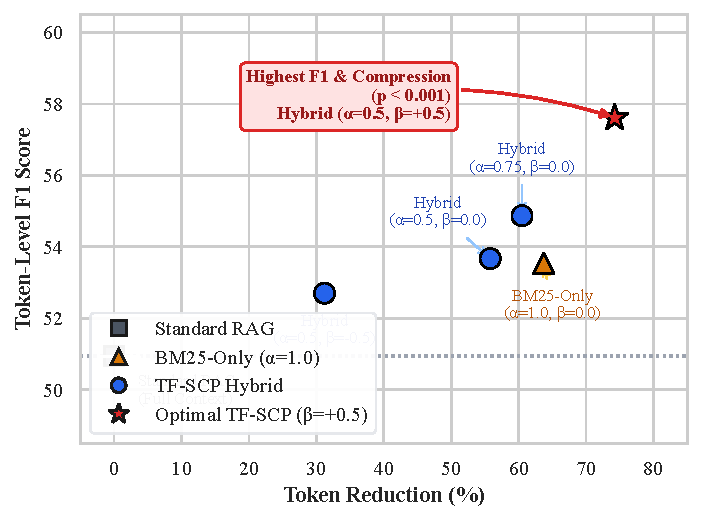
\includegraphics[width=\linewidth]{f1_vs_compression.pdf}
\caption{Context compression vs.\ QA accuracy (token-level F1) across Standard RAG, BM25-only pruning, and TF-SCP hybrid configurations ($n = 1,000$). Aggressive hybrid thresholding ($\alpha=0.5, \beta=+0.5$) achieves the Pareto-dominant optimum.}
\label{fig:f1_vs_compression}
\end{figure}

Scaling to $n = 1,000$ narrows the 95\% bootstrap confidence intervals on F1 from roughly $\pm 8.5$ points (at $n = 100$) to $\pm 2.7$ points (Table~\ref{tab:qa} and Fig.~\ref{fig:f1_vs_compression}). Both primary pruning configurations outperform the full-context baseline on every QA metric, yielding F1 retention of 105.1\% for BM25-only pruning and 105.4\% for TF-SCP hybrid.

Both $\beta = 0.0$ variants cross the nominal $\alpha = 0.05$ threshold on F1: BM25-only gains $+2.60$ F1 ($p = 0.0455$) and TF-SCP hybrid gains $+2.73$ F1 ($p = 0.0255$), although neither passes the stricter Bonferroni threshold of 0.0071. Their EM improvements ($+0.90$, 94 wins vs.\ 85 losses, McNemar $p = 0.550$; and $+2.20$, 92 wins vs.\ 70 losses, McNemar $p = 0.099$) do not reach statistical significance. In the direct paired comparison between the two $\beta = 0.0$ pruners, TF-SCP hybrid and BM25-only are statistically indistinguishable on F1 (53.67 vs.\ 53.54; $\Delta\mathrm{F1} = +0.13$, paired bootstrap $p = 0.901$), while TF-SCP hybrid achieves a highly significant $+4.3$ percentage-point advantage in answer retention (97.5\% vs.\ 93.2\%, exact McNemar $p = 2.6 \times 10^{-12}$).

\subsection{Ablation of the Fusion Weight $\alpha$}

\begin{table*}[t]
\centering
\caption{Sweep of the fusion weight $\alpha$ ($\beta = 0.0$, $n = 1,000$).}
\label{tab:alpha}
\begin{tabular}{@{}lccccccc@{}}
\toprule
$\alpha$ & Token reduction (\%) & Pruning latency (ms) & Answer retained (\%) & EM & F1 & ROUGE-L & F1 retention (\%) \\
\midrule
0.00 (semantic only) & 50.57 & 51.02 & 96.5 & 39.80 & 53.89 & 53.81 & 105.8 \\
0.25 & 52.61 & 51.16 & 97.4 & 40.30 & 53.73 & 53.66 & 105.5 \\
0.50 & 55.79 & 60.61 & 97.5 & 40.40 & 53.67 & 53.59 & 105.4 \\
0.75 & 60.50 & 50.94 & 96.2 & 40.00 & 54.87 & 54.73 & 107.7 \\
1.00 (lexical only) & 63.71 & 13.75 & 93.2 & 39.10 & 53.54 & 53.42 & 105.1 \\
\bottomrule
\end{tabular}
\end{table*}

Token reduction increases monotonically with $\alpha$, from 50.57\% (semantic only) to 63.71\% (lexical only; Table~\ref{tab:alpha}). Answer retention, by contrast, is non-monotonic: it peaks in the interior hybrid region at 97.5\% ($\alpha = 0.50$) and 97.4\% ($\alpha = 0.25$), exceeding both pure semantic pruning (96.5\% at $\alpha = 0.00$) and pure lexical pruning (93.2\% at $\alpha = 1.00$). This confirms genuine complementarity between lexical and dense signals in retaining answer-bearing sentences.

Every $\alpha \in \{0.00, 0.25, 0.50, 0.75, 1.00\}$ achieves a nominally significant F1 gain over Standard RAG ($\Delta\mathrm{F1} = +2.95$ [$p = 0.013$], $+2.79$ [$p = 0.025$], $+2.73$ [$p = 0.025$], $+3.93$ [$p = 0.002$], and $+2.60$ [$p = 0.046$], respectively). Notably, the lexical-weighted hybrid $\alpha = 0.75$ attains 54.87 F1 (107.7\% F1 retention, $\Delta\mathrm{F1} = +3.93$, $p = 0.0022$), which clears the Bonferroni threshold of 0.0071 on F1, although its EM gain (40.00 vs.\ 38.20; 96 wins vs.\ 78 losses, McNemar $p = 0.197$) is not significant. Latency again separates into two regimes: all $\alpha < 1.0$ settings invoke the encoder (50.94--60.61~ms in-situ), whereas $\alpha = 1.00$ requires 13.75~ms.

\subsection{Sensitivity to the Threshold Coefficient $\beta$}

\begin{table*}[t]
\centering
\caption{Sweep of the threshold coefficient $\beta$ ($\alpha = 0.5$, $n = 1,000$).}
\label{tab:beta}
\begin{tabular}{@{}lccccccc@{}}
\toprule
$\beta$ & Token reduction (\%) & Pruning latency (ms) & Answer retained (\%) & EM & F1 & ROUGE-L & $\Delta$F1 vs.\ full ($p$) \\
\midrule
$-$0.50 & 31.20 & 51.94 & 98.8 & 40.00 & 52.70 & 52.63 & $+$1.76 (0.096) \\
0.00 & 55.79 & 60.61 & 97.5 & 40.40 & 53.67 & 53.59 & $+$2.73 (0.025) \\
$+$0.50 & 74.25 & 52.67 & 94.5 & 43.00 & 57.61 & 57.40 & $+$6.67 ($<$0.001) \\
\bottomrule
\end{tabular}
\end{table*}

\begin{figure}[t]
\centering
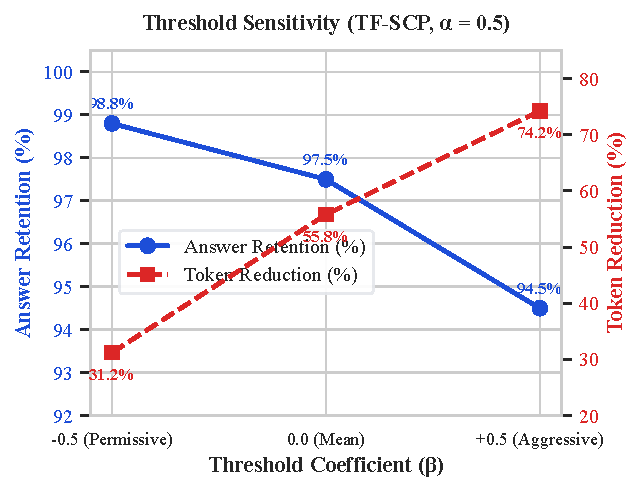
\includegraphics[width=\linewidth]{beta_sensitivity.pdf}
\caption{Trade-off between answer retention (left axis) and token reduction (right axis) as a function of the threshold coefficient $\beta$ for TF-SCP ($\alpha = 0.5, n = 1,000$).}
\label{fig:beta_sensitivity}
\end{figure}

Compression is substantially more sensitive to the threshold coefficient $\beta$ than to the fusion weight $\alpha$ (Table~\ref{tab:beta} and Fig.~\ref{fig:beta_sensitivity}). Raising $\beta$ from $-0.50$ to $+0.50$ increases token reduction from 31.20\% (362.1 tokens, 65.3\% of sentences) to 74.25\% (133.9 tokens, 23.5\% of sentences), lowering generation latency to 511.7~ms and end-to-end latency to 564.3~ms (a 30.1\% end-to-end speed-up over Standard RAG). Answer retention over the same sweep drops from 98.8\% to 94.5\%.

The accuracy advantage of aggressive thresholding observed at $n = 100$ is confirmed as a statistically significant effect at $n = 1,000$ (Fig.~\ref{fig:f1_vs_compression}). At $\beta = +0.50$, TF-SCP achieves the highest performance across all tested configurations: 43.00 EM [40.0, 46.1], 57.61 F1 [55.0, 60.3], and 57.40 ROUGE-L (113.1\% F1 retention). Relative to Standard RAG, both the F1 improvement ($+6.67$ points, paired bootstrap $p = 0.0001$) and the EM improvement ($+4.80$ points; 126 wins vs.\ 78 losses, exact McNemar $p = 0.0010$) remain significant well below the Bonferroni-corrected threshold ($p < 0.0071$). In direct paired comparisons, $\alpha = 0.5, \beta = +0.5$ also significantly outperforms both the default hybrid setting $\alpha = 0.5, \beta = 0.0$ ($\Delta\mathrm{F1} = +3.94, p = 0.0007$; $\Delta\mathrm{EM} = +2.60$, McNemar $p = 0.0422$) and BM25-only pruning $\alpha = 1.0, \beta = 0.0$ ($\Delta\mathrm{F1} = +4.07, p = 0.0001$; $\Delta\mathrm{EM} = +3.90$, McNemar $p = 0.0009$), while simultaneously delivering stronger compression (74.25\% vs.\ 63.71\%) and higher answer retention (94.5\% vs.\ 93.2\%) than BM25-only pruning.

\section{Discussion and Limitations}
\label{sec:discussion}

\subsection{Why the Hybrid Scorer Behaves as Observed}
\label{subsec:hybrid_behavior}

The $n = 1,000$ evaluation clarifies the two opposing mechanisms governing pruned-RAG accuracy: \emph{answer-recall preservation} and \emph{distractor denoising}.

First, semantic fusion functions as an effective recall safeguard. Across the 992 queries where the unpruned context satisfies the boundary-matched answer check, BM25-only pruning ($\alpha = 1.0, \beta = 0.0$) discards the gold answer on 60 queries (totaling 68 non-retained queries including the 8 boundary-artifact cases), whereas TF-SCP hybrid ($\alpha = 0.5, \beta = 0.0$) discards it on only 17 queries (25 total). Query-level overlap shows that 24 missed queries are shared, TF-SCP hybrid rescues 44 of BM25's failures (73.3\% of its 60 genuine losses), and hybrid pruning drops only 1 query missed by BM25-only ($p = 2.6 \times 10^{-12}$, McNemar test). Hybrid fusion at $\alpha = 0.5$ also loses fewer answers than pure semantic pruning at $\alpha = 0.0$ (25 vs.\ 35 total missed; 17 vs.\ 27 genuine losses), because lexical matching guards against rare entity names or numeric spans that dense embeddings under-weight, while MiniLM recovers paraphrastic or indirect phrasing that BM25 misses. Answer loss carries a large accuracy penalty: on queries without the retained answer string, reader F1 falls relative to the full-context reader on the same subsets from 32.4 to 11.2 for BM25-only ($-21.2$ F1), from 33.6 to 20.0 for hybrid $\beta = 0.0$ ($-13.6$ F1), from 42.3 to 15.4 for semantic-only ($-26.9$ F1), and from 34.2 to 19.1 for hybrid $\beta = +0.5$ ($-15.1$ F1).

Second, removing sentences from topically similar hard-negative paragraphs produces a consistent \emph{denoising} gain on the queries whose answer is preserved. Conditioned on answer retention, every pruner outperforms the full-context reader on the exact same queries:
\begin{itemize}
    \item \textbf{BM25-only ($\alpha = 1.0, \beta = 0.0$):} $+4.3$ F1 across 932 queries (56.6 vs.\ 52.3)
    \item \textbf{TF-SCP hybrid ($\alpha = 0.5, \beta = 0.0$):} $+3.1$ F1 across 975 queries (54.5 vs.\ 51.4)
    \item \textbf{Semantic-only ($\alpha = 0.0, \beta = 0.0$):} $+4.0$ F1 across 965 queries (55.3 vs.\ 51.3)
    \item \textbf{TF-SCP hybrid ($\alpha = 0.5, \beta = +0.5$):} $+8.0$ F1 across 945 queries (59.9 vs.\ 51.9)
\end{itemize}

Aggregate $\Delta\mathrm{F1}$ decomposes cleanly into the weighted sum of this denoising benefit and the answer-loss penalty:
\begin{itemize}
    \item \textbf{BM25-only ($\alpha = 1.0, \beta = 0.0$):} $0.932 \times (+4.3) + 0.068 \times (-21.2) = +4.01 - 1.44 = +2.57$ (observed $+2.60$).
    \item \textbf{TF-SCP hybrid ($\alpha = 0.5, \beta = 0.0$):} $0.975 \times (+3.1) + 0.025 \times (-13.6) = +3.02 - 0.34 = +2.68$ (observed $+2.73$).
    \item \textbf{TF-SCP hybrid ($\alpha = 0.5, \beta = +0.5$):} $0.945 \times (+8.0) + 0.055 \times (-15.1) = +7.56 - 0.83 = +6.73$ (observed $+6.67$).
\end{itemize}

This decomposition explains both why BM25-only and TF-SCP hybrid tie on aggregate F1 at $\beta = 0.0$ and why TF-SCP at $\beta = +0.5$ significantly outperforms both. At $\beta = 0.0$, the hybrid pruner keeps 41.2\% of sentences versus 32.7\% for BM25-only; the extra sentences come disproportionately from topical non-answer sentences in the hard negatives that dense similarity scores highly, diluting the denoising gain ($+3.1$ vs.\ $+4.3$ F1) by almost the exact amount saved through fewer answer losses ($-0.34$ vs.\ $-1.44$ F1). However, because the hybrid scorer ranks the gold sentence higher relative to distractors than BM25 alone, shifting the cutoff upward to $\beta = +0.5$ strips away those borderline distractor sentences: token reduction rises to 74.25\%, the denoising gain more than doubles to $+8.0$ F1, and answer loss remains lower than under BM25-only pruning at $\beta = 0.0$ (55 vs.\ 68 non-retained queries). For distraction-sensitive small readers, hybrid scoring combined with a stricter positive threshold ($\beta = +0.5$) captures the recall safeguard of dense fusion without paying the denoising penalty of an overly permissive cutoff. For larger, more distraction-robust readers, the denoising gain should shrink while the penalty for dropping an answer sentence remains large, which would shift the optimal threshold back toward $\beta \le 0.0$; this hypothesis remains to be tested across model scales.

\subsection{Dataset Characteristics Favouring Lexical Scoring}

BM25-only pruning remained competitive at $\beta = 0.0$ partly because of how SQuAD is constructed. Annotators wrote questions while viewing the target paragraph, resulting in high lexical overlap between questions and answer-bearing sentences. Even under those favourable conditions, TF-SCP hybrid reduced genuine answer loss from 6.0\% to 1.7\% (a 4.3 percentage-point retention advantage overall at $\beta = 0.0$, $p = 2.6 \times 10^{-12}$). On corpora with naturally occurring queries---such as Natural Questions or MS MARCO---or multi-hop benchmarks where bridging sentences share few surface terms with the question, the recall disadvantage of pure lexical scoring is expected to widen further.

\subsection{Cost--Benefit of the Semantic Component}

On a commodity CPU, adding the dense encoder increases isolated pruning time from $\approx 11\text{--}14$~ms to $\approx 46.6$~ms (60.6~ms in-situ under contention). Even with this overhead, the 55.8--74.3\% token reduction produces net end-to-end speed-ups of 21.6\% at $\beta = 0.0$ (807.6 $\rightarrow$ 633.2~ms) and 30.1\% at $\beta = +0.5$ (807.6 $\rightarrow$ 564.3~ms), compared with 32.5\% for BM25-only pruning (807.6 $\rightarrow$ 544.8~ms). Crucially, pruning overhead is independent of reader size, whereas LLM prefill latency and API token fees scale with context length and model size. For multi-billion-parameter readers or paid inference endpoints, spending $\approx 35.5$~ms on MiniLM sentence encoding to remove up to 74.3\% of prompt tokens---while significantly improving QA accuracy---becomes progressively more favourable. Several straightforward optimisations were not evaluated here and should further reduce pruning latency:
\begin{itemize}
    \item running or batching the dense encoder on GPU or MPS accelerators;
    \item pre-computing and indexing document-side sentence embeddings offline so only the query is encoded at inference time;
    \item replacing the spaCy dependency parser (10.87~ms) with a lightweight rule-based sentencizer.
\end{itemize}

\subsection{Practical Guidance}

Based on the $n = 1,000$ empirical findings, we recommend:
\begin{enumerate}
    \item \textbf{Precision-optimised default for small readers ($\alpha = 0.5, \beta = +0.5$):} Achieves the best overall trade-off---74.25\% token reduction, a 30.1\% end-to-end speedup, 94.5\% answer retention, and Bonferroni-significant gains of $+6.67$ F1 ($p = 0.0001$) and $+4.80$ EM ($p = 0.0010$) over full-context RAG. The lexical-weighted setting $\alpha = 0.75, \beta = 0.0$ offers an intermediate alternative with a Bonferroni-significant $+3.93$ F1 gain ($p = 0.0022$) and 60.50\% compression.
    \item \textbf{Recall-preserving regime ($\alpha \in [0.25, 0.50], \beta = 0.0$):} Appropriate when minimizing answer-sentence loss is the primary requirement (97.4--97.5\% answer retention, 52.6--55.8\% compression, $+2.73$ to $+2.79$ F1).
    \item \textbf{Ultra-low-latency CPU regime ($\alpha = 1.0, \beta = 0.0$):} Appropriate only when $\approx 14$~ms pruning latency is mandatory, queries exhibit high surface-form overlap with retrieved passages, and a 6.8\% non-retention rate is acceptable.
\end{enumerate}

\subsection{Limitations}

\begin{enumerate}
    \item \textbf{Statistical power across fine-grained ablations.} Scaling to $n = 1,000$ reduced the 95\% F1 confidence interval width to $\pm 2.7$ points and confirmed Bonferroni-significant gains for $\alpha = 0.5, \beta = +0.5$ (both F1 and EM) and $\alpha = 0.75, \beta = 0.0$ (F1). However, the moderate-compression configurations at $\beta = 0.0$ ($\alpha \in \{0.0, 0.25, 0.5, 1.0\}$) achieve only nominal F1 significance ($0.013 \le p \le 0.046$) and non-significant EM differences ($p \ge 0.099$), while pairwise differences along the $\alpha$ sweep ($\le 1.3$ F1 points) remain smaller than the minimum detectable effect at $n = 1,000$.
    \item \textbf{Simulated retrieval.} Every query pool includes the gold paragraph alongside two hard negatives (524.5 tokens total). Production RAG pipelines often process larger candidate pools (e.g., top-5 to top-20 chunks) and sometimes fail to retrieve the gold passage at all; both achievable compression and answer-loss risk will shift under those conditions.
    \item \textbf{Single small reader.} All experiments use a 0.5B-parameter reader (38.20\% EM with full context). Distractor sensitivity---and thus the $+8.0$ F1 denoising gain driving the $\beta = +0.5$ result---may diminish on larger, instruction-hardened models (e.g., 7B--70B parameters).
    \item \textbf{Answerable questions only.} Unanswerable SQuAD v2 queries were excluded, leaving the impact of sentence pruning on abstention and hallucination unmeasured.
    \item \textbf{Metric and retention granularity.} EM and token-F1 penalise valid paraphrases, and normalized substring retention is a coarse proxy: 8 unpruned queries failed the boundary-matched check due to stem/boundary mismatches, and substring matching does not verify whether supporting context sentences were preserved.
    \item \textbf{Sentence independence.} Scoring sentences independently can sever discourse links and coreference antecedents (e.g., pronouns referring to an entity named in a pruned preceding sentence).
    \item \textbf{Hardware specificity of timings.} All timings come from a single Apple M3 laptop CPU, where in-situ pruning (50.9--60.6~ms) ran slower than isolated pruning (46.6~ms) due to contention with reader inference. Absolute speed-ups will vary on server GPUs or API-backed deployments.
    \item \textbf{Scope of baselines.} TF-SCP was benchmarked against its own single-signal ablations and uncompressed RAG. Direct comparisons against trained extractive or perplexity-based compressors (e.g., LLMLingua, RECOMP) are left for future work.
\end{enumerate}

\section{Conclusion}

We presented TF-SCP, a training-free, sentence-level context pruning architecture for Retrieval-Augmented Generation that fuses sparse lexical (BM25) and dense semantic (\texttt{all-MiniLM-L6-v2}) signals via convex linear combination and filters sentences using an adaptive moment-based threshold $\tau = \mu_F + \beta \cdot \sigma_F$. Across a rigorous $n = 1,000$ empirical study on SQuAD v2 with mined hard negatives and a local \texttt{Qwen2.5-0.5B-Instruct} reader, TF-SCP demonstrates that careful post-retrieval sentence filtering eliminates redundant prompt overhead while actively improving answer quality.

Our results expose a clear cost--benefit structure governed by recall preservation and distractor denoising. At $\beta = 0.0$, hybrid scoring ($\alpha = 0.5$) compresses context by 55.79\% and safeguards answer retention at 97.5\%---rescuing 73.3\% of genuine lexical-only answer losses---while incurring only 35.50~ms of isolated dense-encoding overhead on CPU and still cutting end-to-end latency by 21.6\%. Crucially, pairing hybrid scoring with precision-oriented thresholding ($\alpha = 0.5, \beta = +0.5$) proves optimal for compact, distraction-sensitive readers: it compresses context by 74.25\%, accelerates end-to-end inference by 30.1\%, maintains higher answer retention than BM25-only pruning (94.5\% vs.\ 93.2\%), and yields Bonferroni-significant accuracy gains of $+6.67$ F1 ($p = 0.0001$) and $+4.80$ EM ($p = 0.0010$) over uncompressed RAG. Future work will extend this evaluation across larger model families, multi-hop retrieval benchmarks, and offline embedding-cached serving pipelines.

\appendices

\section{Reproducibility and Hyperparameter Specifications}

Table~\ref{tab:repro} summarizes the complete software environment, model checkpoints, prompt templates, and deterministic inference parameters used to generate all results in this paper.

\begin{table}[h]
\centering
\caption{Experimental Environment and Reproducibility Settings.}
\label{tab:repro}
\begin{tabular}{@{}ll@{}}
\toprule
Parameter & Specification \\
\midrule
Hardware & Apple M3 CPU (ARM64), 8~GB unified RAM \\
Operating System & macOS 26.5.1 \\
Python / PyTorch & Python 3.12.12 / PyTorch 2.15.0 \\
Transformers / Datasets & \texttt{transformers} 5.23.0 / \texttt{datasets} 5.2.0 \\
spaCy / Model & \texttt{spacy} 3.8.18 / \texttt{en\_core\_web\_sm} 3.8.0 \\
BM25 / Bi-Encoder Libs & \texttt{rank\_bm25} 0.2.2 / \texttt{sentence-transformers} 6.3.0 \\
Dense Sentence Encoder & \texttt{sentence-transformers/all-MiniLM-L6-v2} \\
Reader LLM & \texttt{Qwen/Qwen2.5-0.5B-Instruct} (FP32, CPU) \\
Decoding Strategy & Greedy (\texttt{do\_sample=False}, \texttt{num\_beams=1}) \\
Generation Limit & \texttt{max\_new\_tokens=32} \\
Dataset / Split & \texttt{rajpurkar/squad\_v2} validation ($n=1,000$) \\
Random Seed & 42 (sampling and document shuffling) \\
Distractors per Query & 2 BM25 hard-negative paragraphs ($M=3$) \\
Minimum Sentences Kept & $k_{\min} = 1$ \\
Numerical Guard & $\varepsilon = 10^{-12}$ \\
\bottomrule
\end{tabular}
\end{table}

For reader inference, prompts follow the native \texttt{Qwen2.5-0.5B-Instruct} chat template with system role \emph{``You are a precise extractive question-answering assistant.''} and user instruction \emph{``Answer the question using only the context below. Reply with the shortest exact phrase from the context that answers the question, with no explanation.''}, followed by the pruned context and question. Outputs are stripped at the first newline and normalized with standard SQuAD punctuation, article, and whitespace rules prior to EM, F1, and ROUGE-L evaluation.

\begin{thebibliography}{99}

\bibitem{lewis2020rag}
P.~Lewis, E.~Perez, A.~Piktus, F.~Petroni, V.~Karpukhin, N.~Goyal, H.~K\"{u}ttler, M.~Lewis, W.-t.~Yih, T.~Rockt\"{a}schel, S.~Riedel, and D.~Kiela, ``Retrieval-augmented generation for knowledge-intensive NLP tasks,'' in \emph{Advances in Neural Information Processing Systems (NeurIPS)}, vol.~33, pp.~9459--9474, 2020.

\bibitem{karpukhin2020dpr}
V.~Karpukhin, B.~Oguz, S.~Min, P.~Lewis, L.~Wu, S.~Edunov, D.~Chen, and W.-t.~Yih, ``Dense passage retrieval for open-domain question answering,'' in \emph{Proc.\ Conf.\ Empirical Methods in Natural Language Processing (EMNLP)}, pp.~6769--6781, 2020.

\bibitem{izacard2021fid}
G.~Izacard and E.~Grave, ``Leveraging passage retrieval with generative models for open domain question answering,'' in \emph{Proc.\ Conf.\ European Chapter of the Association for Computational Linguistics (EACL)}, pp.~874--880, 2021.

\bibitem{liu2024lost}
N.~F.~Liu, K.~Lin, J.~Hewitt, A.~Paranjape, M.~Bevilacqua, F.~Petroni, and P.~Liang, ``Lost in the middle: How language models use long contexts,'' \emph{Transactions of the Association for Computational Linguistics (TACL)}, vol.~12, pp.~157--173, 2024.

\bibitem{shi2023distracted}
F.~Shi, X.~Chen, K.~Misra, N.~Scales, D.~Dohan, E.~H.~Chi, N.~Sch\"{a}rli, and D.~Zhou, ``Large language models can be easily distracted by irrelevant context,'' in \emph{Proc.\ Int.\ Conf.\ Machine Learning (ICML)}, pp.~31210--31227, 2023.

\bibitem{mallen2023not}
A.~Mallen, A.~Asai, V.~Zhong, R.~Das, D.~Khashabi, and H.~Hajishirzi, ``When not to trust language models: Investigating effectiveness of parametric and non-parametric memories,'' in \emph{Proc.\ Annu.\ Meeting Assoc.\ Comput.\ Linguistics (ACL)}, pp.~9802--9822, 2023.

\bibitem{cuconasu2024noise}
F.~Cuconasu, G.~Trappolini, F.~Siciliano, S.~Filice, C.~Campagnano, Y.~Maarek, N.~Tonellotto, and F.~Silvestri, ``The power of noise: Redefining retrieval for RAG systems,'' in \emph{Proc.\ Int.\ ACM SIGIR Conf.\ Research and Development in Information Retrieval}, pp.~719--729, 2024.

\bibitem{robertson2009bm25}
S.~Robertson and H.~Zaragoza, ``The probabilistic relevance framework: BM25 and beyond,'' \emph{Foundations and Trends in Information Retrieval}, vol.~3, no.~4, pp.~333--389, 2009.

\bibitem{reimers2019sbert}
N.~Reimers and I.~Gurevych, ``Sentence-BERT: Sentence embeddings using Siamese BERT-networks,'' in \emph{Proc.\ Conf.\ Empirical Methods in Natural Language Processing (EMNLP)}, pp.~3982--3992, 2019.

\bibitem{wang2020minilm}
W.~Wang, F.~Wei, L.~Dong, H.~Bao, N.~Yang, and M.~Zhou, ``MiniLM: Deep self-attention distillation for task-agnostic compression of pre-trained transformers,'' in \emph{Advances in Neural Information Processing Systems (NeurIPS)}, vol.~33, pp.~5776--5788, 2020.

\bibitem{nogueira2019passage}
R.~Nogueira and K.~Cho, ``Passage re-ranking with BERT,'' \emph{arXiv preprint arXiv:1901.04085}, 2019.

\bibitem{ma2021replication}
X.~Ma, K.~Sun, R.~Pradeep, and J.~Lin, ``A replication study of dense passage retriever,'' \emph{arXiv preprint arXiv:2104.05740}, 2021.

\bibitem{cormack2009rrf}
G.~V.~Cormack, C.~L.~A.~Clarke, and S.~Buettcher, ``Reciprocal rank fusion outperforms Condorcet and individual rank learning methods,'' in \emph{Proc.\ Int.\ ACM SIGIR Conf.\ Research and Development in Information Retrieval}, pp.~758--759, 2009.

\bibitem{li2023selective}
Y.~Li, B.~Dong, F.~Guerin, and C.~Lin, ``Compressing context to enhance inference efficiency of large language models,'' in \emph{Proc.\ Conf.\ Empirical Methods in Natural Language Processing (EMNLP)}, pp.~6342--6353, 2023.

\bibitem{jiang2023llmlingua}
H.~Jiang, Q.~Wu, C.-Y.~Lin, Y.~Yang, and L.~Qiu, ``LLMLingua: Compressing prompts for accelerated inference of large language models,'' in \emph{Proc.\ Conf.\ Empirical Methods in Natural Language Processing (EMNLP)}, pp.~13358--13376, 2023.

\bibitem{jiang2024longllmlingua}
H.~Jiang, Q.~Wu, X.~Luo, D.~Li, C.-Y.~Lin, Y.~Yang, and L.~Qiu, ``LongLLMLingua: Accelerating and enhancing LLMs in long context scenarios via prompt compression,'' in \emph{Proc.\ Annu.\ Meeting Assoc.\ Comput.\ Linguistics (ACL)}, pp.~1658--1677, 2024.

\bibitem{pan2024llmlingua2}
Z.~Pan, Q.~Wu, H.~Jiang, M.~Xia, X.~Luo, J.~Zhang, Q.~Lin, V.~R\"{u}hle, Y.~Yang, C.-Y.~Lin, H.~V.~Zhao, L.~Qiu, and D.~Zhang, ``LLMLingua-2: Data distillation for efficient and faithful task-agnostic prompt compression,'' in \emph{Findings of the Association for Computational Linguistics (ACL)}, pp.~963--981, 2024.

\bibitem{xu2024recomp}
F.~Xu, W.~Shi, and E.~Choi, ``RECOMP: Improving retrieval-augmented LMs with context compression and selective augmentation,'' in \emph{Proc.\ Int.\ Conf.\ Learning Representations (ICLR)}, 2024.

\bibitem{wang2023filco}
Z.~Wang, J.~Araki, Z.~Jiang, M.~R.~Parvez, and G.~Neubig, ``Learning to filter context for retrieval-augmented generation,'' \emph{arXiv preprint arXiv:2311.08377}, 2023.

\bibitem{rajpurkar2018squad2}
P.~Rajpurkar, R.~Jia, and P.~Liang, ``Know what you don't know: Unanswerable questions for SQuAD,'' in \emph{Proc.\ Annu.\ Meeting Assoc.\ Comput.\ Linguistics (ACL)}, pp.~784--789, 2018.

\bibitem{lin2004rouge}
C.-Y.~Lin, ``ROUGE: A package for automatic evaluation of summaries,'' in \emph{Text Summarization Branches Out (ACL Workshop)}, pp.~74--81, 2004.

\bibitem{qwen2024qwen25}
Qwen Team, ``Qwen2.5: A party of foundation models,'' Technical Report, 2024. [Online]. Available: \url{https://qwenlm.github.io/blog/qwen2.5/}

\end{thebibliography}

\end{document}
